% Created 2021-11-18 Thu 20:50
% Intended LaTeX compiler: pdflatex
\documentclass[11pt]{article}
\usepackage[utf8]{inputenc}
\usepackage[T1]{fontenc}
\usepackage{graphicx}
\usepackage{grffile}
\usepackage{longtable}
\usepackage{wrapfig}
\usepackage{rotating}
\usepackage[normalem]{ulem}
\usepackage{amsmath}
\usepackage{textcomp}
\usepackage{amssymb}
\usepackage{capt-of}
\usepackage{hyperref}
\author{190022658}
\date{\today}
\title{CS3104 P2 - Scheduling Analysis}
\hypersetup{
 pdfauthor={190022658},
 pdftitle={CS3104 P2 - Scheduling Analysis},
 pdfkeywords={},
 pdfsubject={},
 pdfcreator={Emacs 27.2 (Org mode 9.5)}, 
 pdflang={English}}
\begin{document}

\maketitle

\section{Part 1 - BSD scheduler summary}
\label{sec:orgb21416b}
\begin{description}
\item[{NOTE}] Used NetBSD as example.\\
\end{description}
\subsection{Scheduling algorithm}
\label{sec:orgb4f3a74}
The traditional 4.4BSD scheduler employs a \textbf{multi-level feedback queues} algorithm, favoring interactive, short-running threads to CPU-bound ones.\\

In multi-level feedback queues algorithm, processes are classified into groups and each group has a queue for themselves. Unlike multi-level queues, multi-level feedback queues 'learn' from the past i.e. move the processes between groups based on run-time characteristics. The algorithm chooses from the highest (non-empty) priority queue.\\

The system adjusts the priority dynamically to reflect resource requirements (e.g., being blocked awaiting an event) and the amount of resources consumed by the thread (e.g., CPU time). Threads are moved between run queues based on changes in their scheduling priority (hence the word feedback in the name multilevel feedback queue). When a thread other than the currently running thread attains a higher priority (by having that priority either assigned or given when it is awakened), the system switches to that thread immediately if the current thread is in user mode.\\

In the BSD scheduler, the priority queues uses the round-robin algorithm for scheduling.\\

In general, if the time quantum is short, the interactive response will be better. But longer time quanta provide higher system throughput because the system will have less overhead from doing context switches. Based on this, the time quantum used in the BSD scheduler is 0.1 seconds.\\

\subsection{Priorities}
\label{sec:org32b7c91}
The process priority depends on two values: kg\_estcpu and kg\_nice\\
\begin{itemize}
\item p\_estcpu provides an estimate of the recent CPU utilization of the process\\
\item p\_nice is a user-settable weighting factor that ranges numerically between -20 and 20. The normal value for kg\_nice is 0 (does not affect the process priority). Negative values increase a thread's priority, whereas positive values decrease its priority.\\
\end{itemize}
A thread's user-mode scheduling priority is calculated after every four clock ticks (typically 40 milliseconds) that it has been found running by this equation:\\
p\_usrpri = PUSER + (p\_estcpu / 4) + 2 p\_nice\\

Values less than PUSER are set to PUSER and values greater than 127 are set to 127 (in case of NetBSD).\\

The p\_estcpu is adjusted for every one second via a digital decay filter (reduces the value of p\_estcpu).\\

\subsection{Process run queues}
\label{sec:orgb9fd61e}
In freeBSD, there are 32 queues and each queue has 4 priority processes (since the scheduling priority ranges from 0 to 127).\\

The run queues contain all the runnable process in main memory except the currently running process. The head of each run queue is kept in an array which is associated with a bitmap, \emph{whichqs}. \emph{whichqs} is used to identify the non-empty run queues.\\

The queues are managed by\\
\begin{itemize}
\item setrunqueue()\\
\item rmrq()\\
\end{itemize}

The context switch is divided into two types\\
\begin{itemize}
\item miswitch()  - machine independent\\
\item cpuswitch() - machine dependent\\

\item cpuswitch() - responsible for selecting a new process to run\\
\begin{enumerate}
\item Blocks interrupts, then looks for a non-empty queue (by finding the first non-zero bit in the \emph{whichqs} bit vector). If there are no non-empty queues, there are no processes to run, so unblocks interrupts and (idle) loop i.e. waits for a process.\\
\item Given a non-empty queue, remove the first process on the queue\\
\item If the queue is now empty, change the appropriate bit in \emph{whichqs}.\\
\item Clear the \emph{curproc} pointer (references the currently running process) and the \emph{want\_resched} flag (shows that a context-switch should take place).\\
\item Set the new process running and unblock interrupts.\\
\end{enumerate}

\item miswitch() - called when a process wants to \emph{sleep()}\\
\end{itemize}

Voluntary context switches occur when a process calls the sleep() routine.\\
Sleep() can be invoked by only a runnable process, so sleep() needs only to place the process on a sleep queue and to invoke mi\_switch() to schedule the next process to run. \emph{mi\_switch()} can’t be called by a process that is in interrupt state, because it must be called with in the context of a running process.\\

Often an interrupt thread will not want to sleep() itself but will be delivering data that will cause the kernel to want to run a different thread than the one that was running before the interrupt. Thus, the kernel needs a mechanism to request that an involuntary context switch be done at the conclusion of the interrupt.\\

The new mechanism is handled by the machine-dependent need\_resched() routine, which generally sets a global reschedule request flag, named want\_resched, and then posts an asynchronous system trap (AST) for the current process. An AST is a trap that is delivered to a thread the next time that that thread is preparing to return from an interrupt, a trap, or a system call. Some architectures support ASTs directly in hardware; other systems emulate ASTs by checking an AST flag at the end of every system call, trap, and interrupt. When the hardware AST trap occurs or the AST flag is set, the mi\_switch() routine is called, instead of the current thread resuming execution. When a process is woken up and if it comes across an AST trap it requests for reschedule instead of resuming the process execution.\\

\subsection{Pre-emtive}
\label{sec:orgdcf5a49}
The scheduler pre-empts when a user process gains higher priority than the running process. The 4.4 BSD scheduler doesn’t support preemptions in kernel mode.\\
\subsection{Multi-core}
\label{sec:org5377abc}
The BSD scheduler was designed for uniprocessor systems. It continues to work well in multi-core environments but the new ULE and M2 schedulers are optimized for those environments.\\


\section{Part 2 - Profiling}
\label{sec:orgfd3b1aa}
The code is modified to print each system call start and end time seperated by a comma and print a new line after. This outputs a csv value which is redirected into a file by a bash command.\\

There are 3 folders containing code for the 3 I/O profiles exhibited\\

\begin{figure}[htbp]
\centering
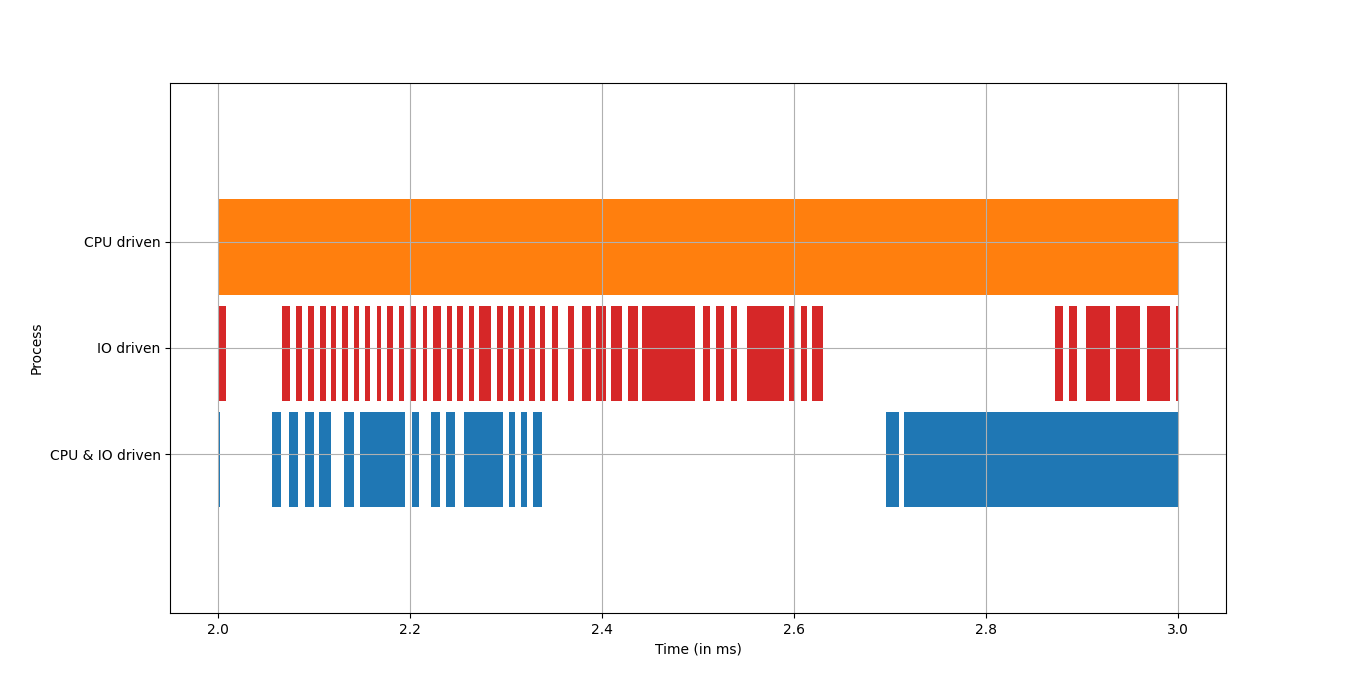
\includegraphics[width=.9\linewidth]{./Part2-CPUBursts.png}
\caption{CPU Bursts}
\end{figure}

\begin{enumerate}
\item Computation-driven\\
'cpudriven'\\
For a CPU driven program, using the Ackermann function seemed like a good idea, but it is hard to control the length of the program run time. Another idea was to calculate the numbers of PI.\\

I chose to generate prime numbers without any optimizations. I can control the run time here by changing the number to loop up to to calculate the prime number.\\

These were viable options because they don't rely on system calls and don't use any libraries (which might use system calls). These are mathematical options.\\

Notice that in Figure 1, there is only a cpu burst that goes on for the whole duration. That is because the program has no external (or I/O) requirements.\\

\begin{figure}[htbp]
\centering
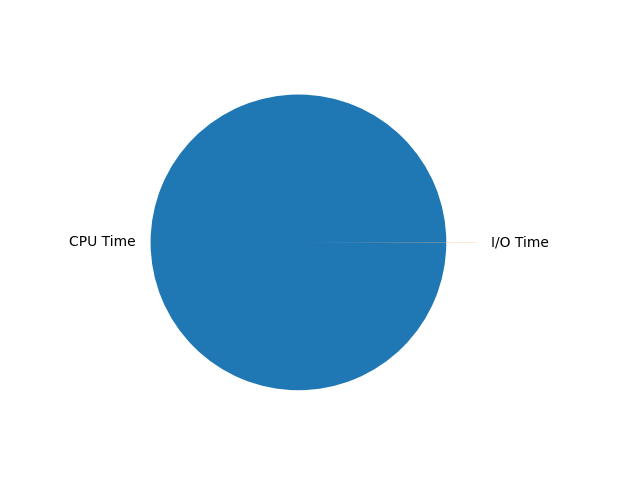
\includegraphics[width=.9\linewidth]{./CPUTimeDist.png}
\caption{CPU Driven Process time distribution}
\end{figure}

\item I/O-driven\\
'iodriven'\\
For a I/O driven program, I created a file with 5000 lines of text and made a program that would open it and count the number of characters then close it. To control the length of time that the program runs, I looped the previous steps until the desired time reached.\\

In Figure 1, there are cpu and io bursts alike but there are more io bursts. That is because the program has to use system calls to access the file and read the characters.\\

\begin{figure}[htbp]
\centering
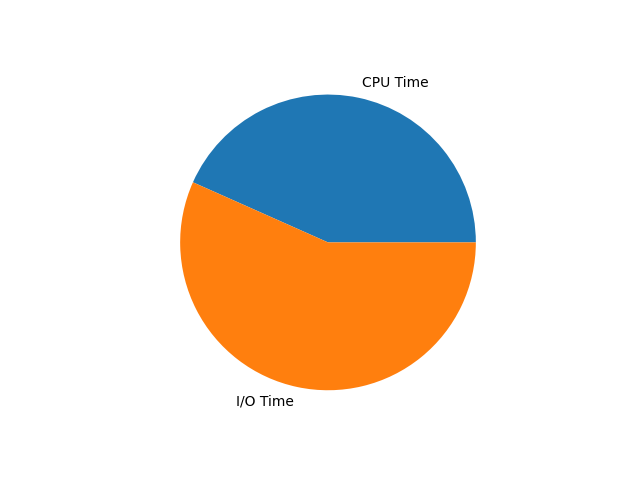
\includegraphics[width=.9\linewidth]{./IOTimeDist.png}
\caption{IO Driven Process time distribution}
\end{figure}

\item CPU \& IO-driven\\
'cpu\&iodriven'\\
For a CPU \& IO driven program, I wrote a program to generate prime numbers and write it to a file.\\

In Figure 1, there are cpu and io bursts alike and they are almost equal. The overall time shows better that the time spent doing I/O is midway to that of CPU driven and IO driven. That is because the program has to use system calls to access the file and has to do computation to generate prime numbers.\\

\begin{figure}[htbp]
\centering
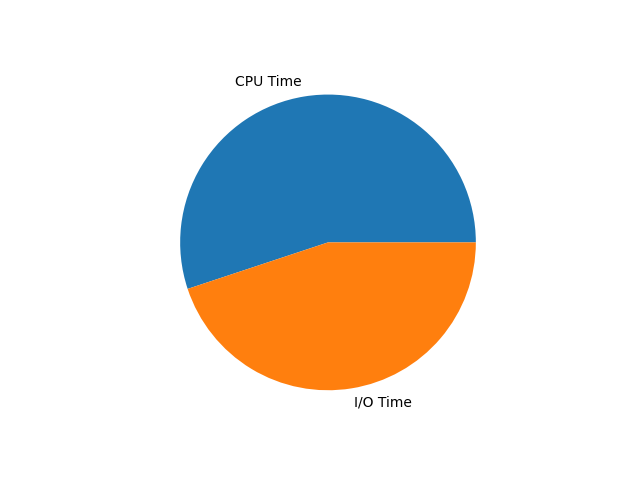
\includegraphics[width=.9\linewidth]{./CPU&IOTimeDist.png}
\caption{CPU \& IO Driven Process time distribution}
\end{figure}
\end{enumerate}


\section{Part 3 - Analysis}
\label{sec:org3979a42}
\begin{figure}[htbp]
\centering
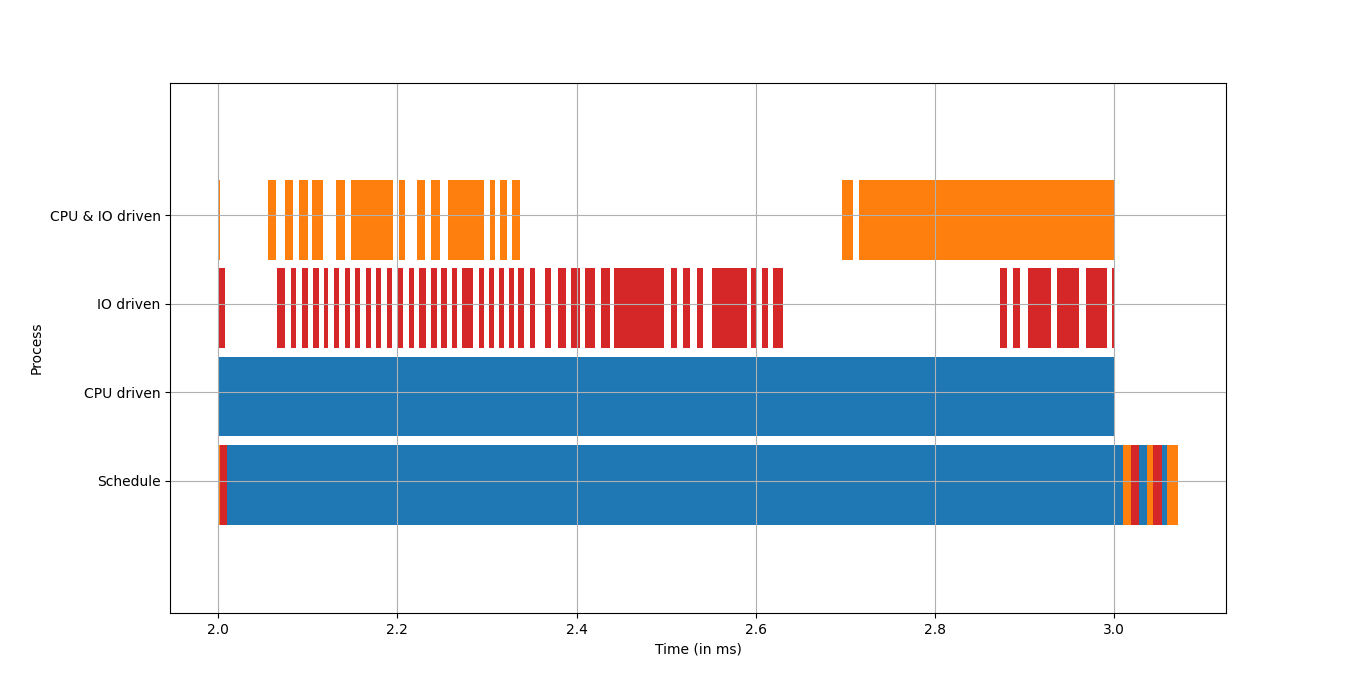
\includegraphics[width=.9\linewidth]{./Scheduled.png}
\caption{Schedule}
\end{figure}

The algorithm is basically a fcfs since the bursts are never longer than 100ms. I could have made a program to generate the graph but since it was only 10 steps, I decided not to.\\

\subsection{Steps:}
\label{sec:org72d10d6}
Run cpu burst (1st process)\\
sleep()\\
switch()\\
Run cpu burst (2nd process)\\
sleep()\\
switch()\\
Run cpu burst (3rd process)\\
(a burst from the 1st process queues)\\
(a burst from the 2nd process queues)\\
3rd Process ends\\
Run cpu burst (1st process)\\
and so on\ldots{}\\
all processes end\\
if there are no processes left edit \emph{whichqs}\\


\section{Part 4}
\label{sec:orgb8aca31}
\begin{itemize}
\item The Process Control Block is stored in a struct called \emph{proc}.\\
\begin{itemize}
\item It contains data like p\_estcpu and p\_usrpri from part 1. These are used when calculating priority in \emph{setpriority()}.\\
\item \emph{p\_usrpri} is calculated in \emph{schedcpu()} like you'd expect because it recomputes process priority every second.\\
\item \emph{p\_usrpri} is updated in \emph{schedclock()} to favor processes which haven't been run recently.\\
\end{itemize}

\item PCBs are stored on the run queue using \emph{setrunqueue()} function\\

\item In \emph{roundrobin()}, if the process has seen roundrobin then it should yield.\\

\item According to me, on line number 241 \emph{schedcpu()} checks if the process is running and removes and adds it to the tail of the list if there's a process with higher priority.\\
\end{itemize}


\section{Bibliography}
\label{sec:orgea2c841}
\begin{itemize}
\item \url{https://www.scs.stanford.edu/15wi-cs140/pintos/pintos\_7.html}\\
\item \url{https://manikishan.wordpress.com/2020/05/10/scheduling-in-netbsd-part-1/}\\
\item \url{https://flylib.com/books/en/2.849.1.57/1/}\\
\item \url{https://github.com/openbsd/src/blob/master/sys/kern/kern\_sched.c}\\
\item \url{https://www.informit.com/articles/article.aspx?p=366888\&seqNum=4}\\
\item Operating Systems Concepts Essentials 2nd Edition - Abraham Silberschatz, Peter Baer Galvin, Greg Gagne\\
\end{itemize}
\end{document}
